\documentclass[tikz,border=12pt]{standalone}
\usepackage{stix}
\usepackage{tikz}
\usetikzlibrary{angles}
\usetikzlibrary{quotes}
\usepackage{tkz-euclide}
\usetkzobj{all}
\usetikzlibrary{arrows, arrows.meta}
\definecolor{blue}{RGB}{0,51,255}
\definecolor{green}{RGB}{0,153,0}
\begin{document}
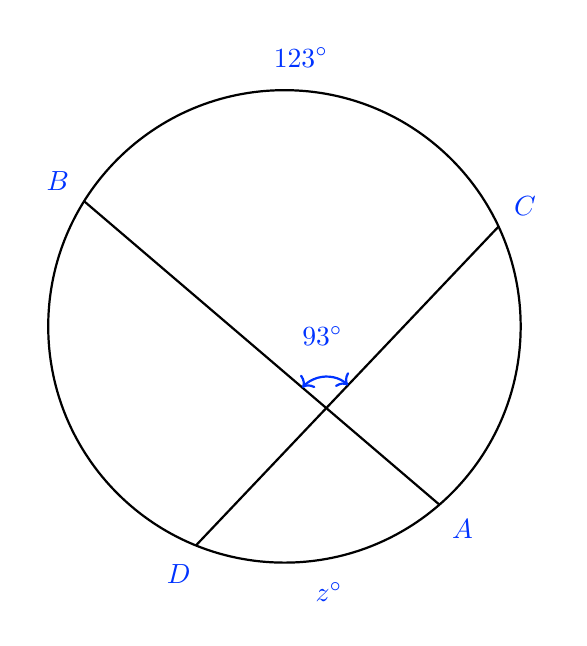
\begin{tikzpicture}
\begin{scope}[>={Stealth[scale=1.2]} , thick,rotate=0]

\coordinate (M) at (0,0);
\coordinate (A) at (311:3);
\coordinate (D) at (248:3);
\coordinate (B) at (148:3);
\coordinate (C) at (25:3);
\coordinate (x1) at (86.5:3);
\coordinate (x2) at (279.5:3);

\path pic ["$A$", blue, angle radius=20]  {angle = D--A--C};
\path pic ["$B$", blue, angle radius=20]  {angle = C--B--D};
\path pic ["$C$", blue, angle radius=20]  {angle = A--C--B};
\path pic ["$D$", blue, angle radius=20]  {angle = B--D--A};
\path pic ["$123^{\circ{}}$", blue, angle radius=20]  {angle = C--x1--B};
\path pic ["$z^{\circ{}}$", blue, angle radius=20]  {angle = D--x2--A};



\coordinate (x) at (intersection of C--D and A--B);

\draw (0,0) circle (3cm);
\draw(A)--(B);
\draw(D)--(C);

\pic [blue,draw,{To}-{To}, angle radius=0.4cm,angle eccentricity=2.3
,"$93^{\circ{}}$"] {angle = C--x--B};


\end{scope}
\end{tikzpicture}
\end{document}